\chapter*{Projekt aplikacji}
Aplikacja jest wysoce wyspecjalizowana -- przeprowadza wyłącznie proces symulacji i uczenia. Użytkownik może konfigurować ustawienia tego procesu.
\section*{Wymagania funkcjonalne}
\begin{itemize}
	\item Przeprowadzanie procesu uczenia optymalnych czasów świecenia sygnalizatorów na skrzyżowaniu za pośrednictwem algorytmu ewolucyjnego, wykorzystującego symulację ruchu pojazdów do oceny rozwiązań, 
	\item Konfiguracja ustawień symulacji, będącej bazą procesu uczenia,
	\item Konfiguracja ustawień algorytmu ewolucyjnego,
	\item Wyświetlanie na bieżąco informacji o przebiegu uczenia,
	\item Wyświetlenie wyników uczenia po jego zakończeniu.
\end{itemize}
\section*{Wymagania pozafunkcjonalne}
\begin{itemize}
	\item Stabilność -- aplikacja musi pracować bezawaryjnie przez wiele godzin,
	\item Wydajność -- aplikacja musi działać na tyle wydajnie, aby symulacja mogła być przeprowadzana kilkadziesiąt razy szybciej niż czas rzeczywisty.
\end{itemize}
\section*{Przypadki użycia}
W projekcie występuje tylko jeden przypadek użycia: ,,Przeprowadź proces optymalizacji sygnalizacji świetlnej''. Przedstawia go diagram aktywności na rysunku~\ref{fig:diagramaktywnosci}. 
\section*{Przebieg przypadku użycia ,,Przeprowadź proces optymalizacji sygnalizacji świetlnej''}
Użytkownik najpierw może ustawić konfigurację symulacji oraz algorytmu ewolucyjnego. Następne wybiera scenariusz (czyli kolejność zapalania sygnalizatorów), co powoduje rozpoczęcie procesu uczenia. Aplikacja kolejno generuje, symuluje, a potem ocenia osobników pokolenia, jednocześnie wyświetlając na ekranie informacje o przebiegu uczenia. Pokolenia są kolejno generowane tak długo, aż zostanie osiągnięta ich liczba określona w konfiguracji. Następnie aplikacja wyświetla ekran końcowy prezentujący wyniki uczenia.
\begin{figure}[H]
	\centering
	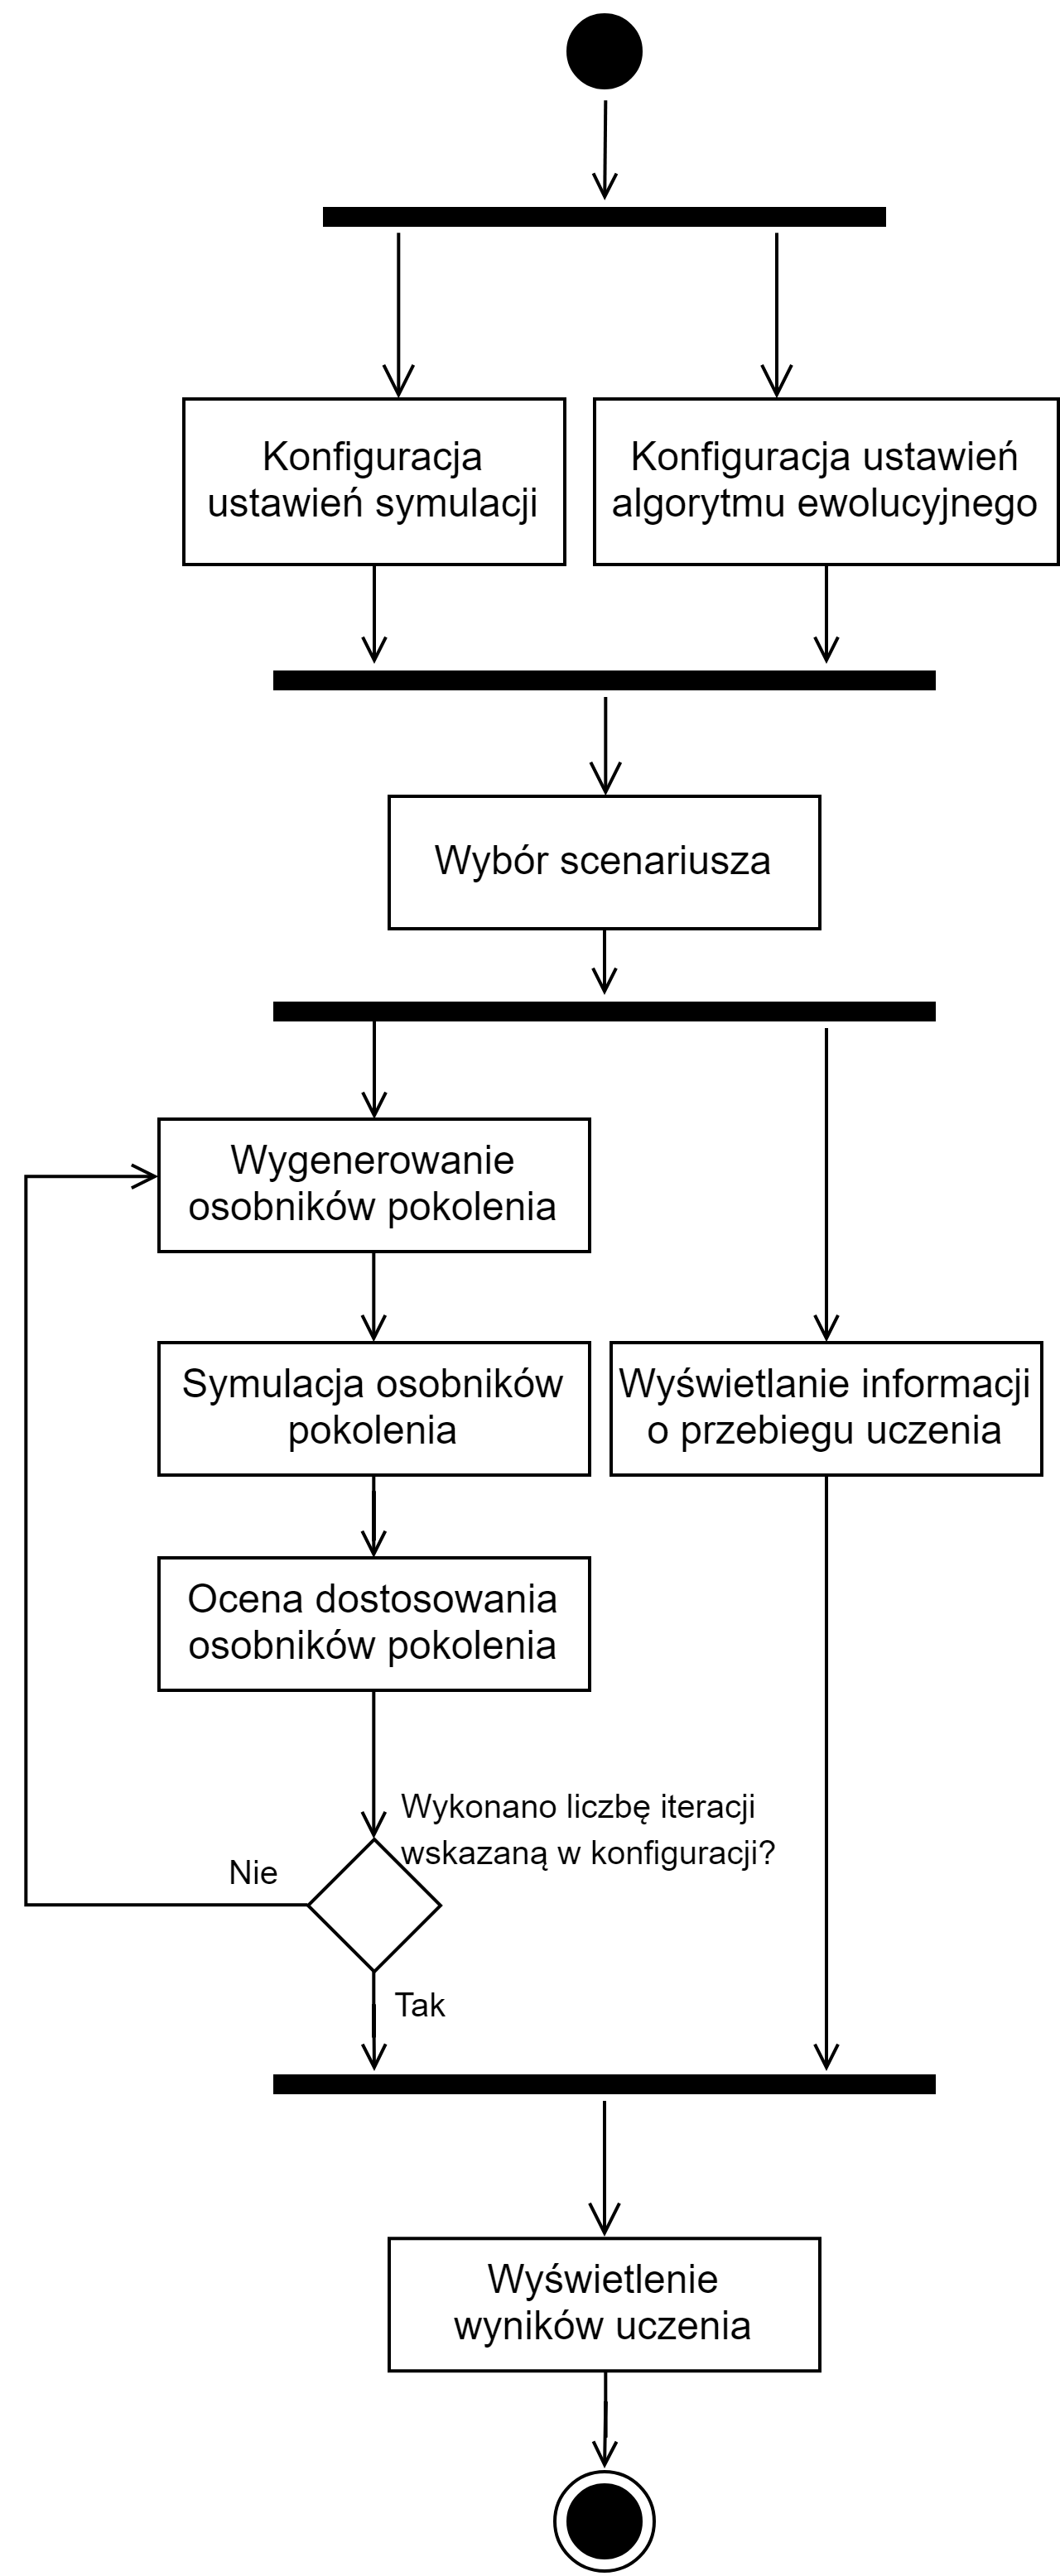
\includegraphics[height=0.8\textheight]{diagram_aktywnosci}
	\caption[Diagram aktywności przypadku użycia ,,Przeprowadź proces uczenia sygnalizacji'']{Diagram aktywności przypadku użycia ,,Przeprowadź proces uczenia sygnalizacji''}
	\label{fig:diagramaktywnosci}
\end{figure}
